\section{Preliminaries}
In this section, we first introduce the preliminaries for both scenarios.
In the first step, we preprocess the interest profiles and tweet streams. 

In the query side,
We first obtain external resources for each user interest profile.
Using the Google search API, 
we obtain the top five items which is consisting of titles and snippets for each interest profile,
then we combine the titles and snippets to generate a background context document for each interest profile.
In addition, we incorporate the context document with original interest profile through linear interpolation. 

In the tweet stream side,
our system will monitor the Twitter's live tweet sample stream continuously using the official API.
As soon as the system obtains the json data of tweets,
the system will preprocess the tweet text and filter non-English tweets or words.
To boost the speed of identifying candidate tweets for each user's interest profile, 
for each interest profile $q$, 
we simply filter tweets that do not contain keywords for $q$,
and the rest tweets are chosen as candidate tweet collection $\Gamma$ for $q$.

In the following step, we will utilize a query-biased filtering method to choose pushed tweets from the candidate tweet collection $\Gamma$ for each interest profile every day.
In order to push novel tweets for each topic in different days, we maintain a collection consisting of tweets which have been pushed in previous time for each interest profile. Besides, we make a binary classifier to judge the tweets' novelty against the corresponding collection.

\subsection{Preprocessing}
The preprocessing we adopt on the queries and tweet stream is described as follows:
\begin{itemize}
\item \textbf{Non-English Filtering:} We discard the non-English tweets according to the result of twitter's language detector.
\item \textbf{Non-English Words:} We simply filter the words which contain non-ASCII characters.
\item \textbf{Simple Retweet Additional Commentary Elimination:} We eliminate the additional commentary of tweets that contains 'RT @' with the consideration that all retweets should be normalized to the underlying tweets according to the guideline.
\item \textbf{Porter Stemming and Stopword Filtering:} Stopwords are removed from these tweets using InQuery stopwords list. These tweets are stemmed using the Porter Algorithm.
% such as the number of a vertex's neighbors which have been added in previous clusters.
\end{itemize}

\subsection{Query Expansion}
As microblog retrieval suffers severely from the vocabulary mismatch problem
(i.e. term overlap between query and tweet is relatively small),
query expansion techniques can be leveraged to improve the retrieval effectiveness \cite{zhai2011mbfb}.
In this section, we introduce the method on the basis of query expansion.

To better describe the query expansion, 
we first name the original user interest profile (namely query) offered by TREC'2015 \emph{OriginQuery}.
Here we only use the topic keywords of each interest profile since we utilize external web resources to depict the background information of the given profile.
For a certain \emph{OriginQuery},
we submit the query to Google Search Engine API. 
Non and verb terms from the titles and snippets of returned top five documents to generate a new query (i.e. \emph{WebQuery}). 
Then we generate the \emph{MergeQuery} by interpolating the \emph{OriginQuery} and \emph{WebQuery}.
\begin{equation}
\label{equ:merge}
\emph{MergeQuery} = \alpha \cdot \emph{OriginQuery} + (1-\alpha) \cdot \emph{WebQuery}
\end{equation}

Then we utilize the updated query to represent original interest profile and then estimate the relevance between the query and tweets.
\begin{figure}[htbp]
\centering
{
	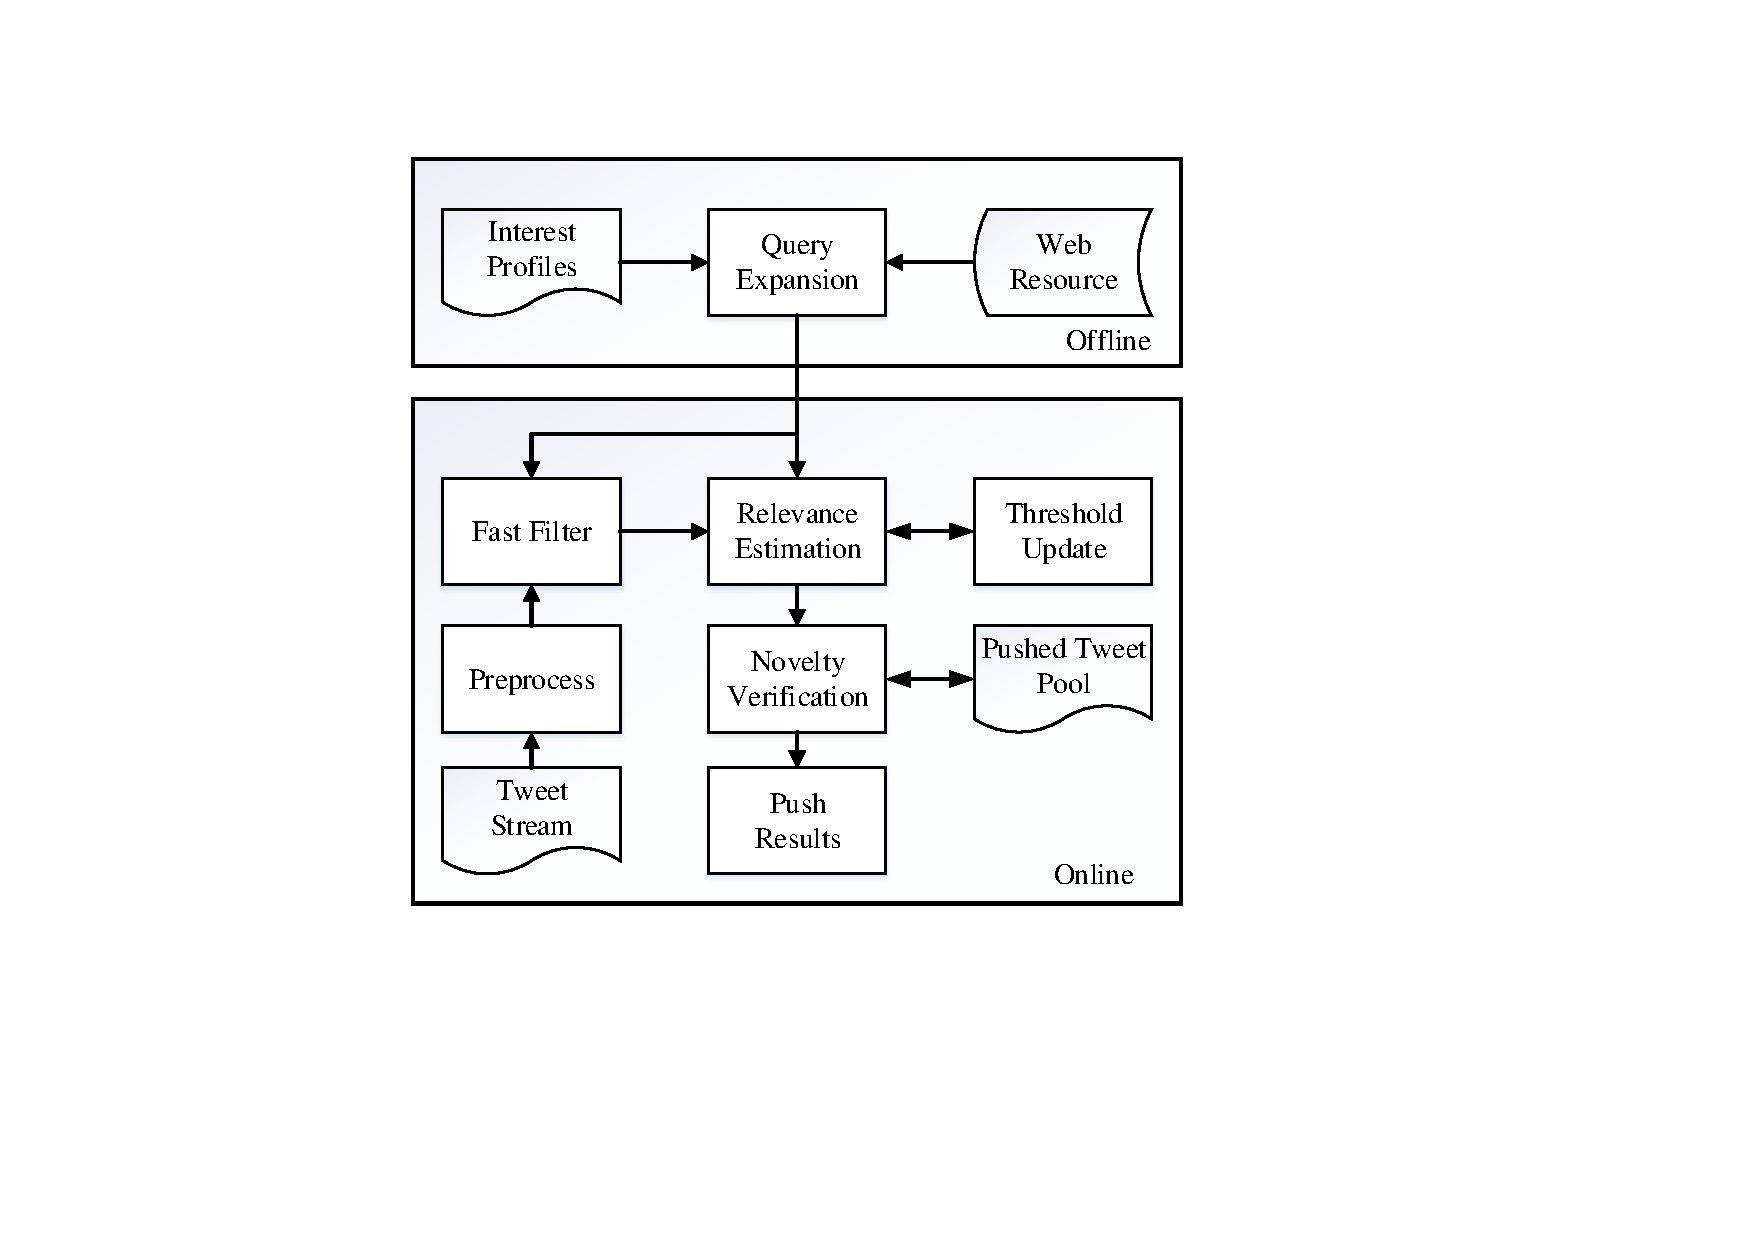
\epsfig{file=figures/scenarioA.pdf,width=0.45\textwidth}
}
\caption{Scenario A System Framework.}
\label{fig:Asys}
\end{figure}
